\section{Background}
\label{sec:background}

% Link Prediction refers to finding missing links in a graph Link prediction in social and gaming networks has been studied for a while now. 
% The Link Prediction problem has been well studied in n

\paragraph{Problem} Formally, the link prediction problem for a given graph $G(V,
E)$ at time t, where $V$ represents the Vertices set and $E$ represents the
Edge set is predicting edges that would form at time $t' (> t)$ between nodes
in $G$ which had no edge at time $t$.  There are several approaches that have
been studied for Link Prediction in single and multiplex networks.


\subsection{Single layer link prediction}
\label{sec:slp}

Many graphs such as social networks or gaming networks can be modelled as a
single layer in which  nodes and edges are of one type. The first ever link
prediction study in social networks was done by Nowell et.
al~\cite{liben2007link} using several  node based and path based metrics. To
summarize, node based metrics include \texttt{Common neighbours},
\texttt{Jaccard's coefficient}, \texttt{Adamic Adar} whereas the path based
metrics include \texttt{Shortest Path Distance} and \texttt{PageRank}. Hasan
et al.~\cite{al2006link} extended this work  by using supervised learning
techniques by taking the node and path based similarity scores as features
apart from  external contextual features. Also, a number of statistical methods 
and probablistic modelling methods have been used to do the same - for more 
details see the survey~\cite{al2011survey}. 

Typically any method which works for static link prediction can be used
directly for link prediction in dynamic networks. A simple way to do this is to
aggregate the graph snapshots $G_i(V_i, E_i)$ at all  times $t_i(< t)$ and
predict whether a new link might form at time $t'$. However,  this method
does not account for seasonal changes in link formation. As a solution,  Sarkar
et. al~\cite{sarkar2012nonparametric} implemented a non- parametric link
prediction  algorithm for a sequence of given snapshots over time. They do not
aggregate the graph snapshots for  link prediction, instead, they find a
snapshot with very similar characteristics to the current one from the past
and use its evolution to predict links for the current graph. However, their
method wont be applicable in situations where there is less data on the past.
So, in our work, we use simple aggregation of graph snapshots instead of using the
non-parametric algorithm since we have limited past data.

% Link prediction in
% such graphs can be defined as prediciting a possiblity of  an edge in future
% between two nodes for which there exists no edge currently. 

% For Eg: In Facebook, friendship graph is a single layer graph with 
% nodes being friends and edges representing friendship. 

% Link prediction in social

% A paragraph or two about single layer link prediction and its methodologies in
% general. 

\subsection{Multi layer link prediction}
\label{sec:mlp}

The primay motive of link prediction in multiplex networks is to leverage
cross-layer information to improve the accuracy. Davis et.
al~\cite{davis2013supervised} attempts to do this by using a probabilistically
weighted  extension of Adamic/Adar measure i.e., they use a popular method
called triad consensus to reweight the  edges of a graph. Then they do
supervised  learning by using the extended Adamic/Adar score and other
unsupervised metrics as features. This method, however, doesn't incorporate
temporal information. Hajibagheri et. al~\cite{hajibagheri2016holistic} tried
to incorporate  temporal information by changing the weights of the target
layer using all past graph snapshots and using a decay function to give more weight
to the recent snapshots. The reweighting algorithm is shown in
figure~\ref{fig:algo1}.

\begin{figure}[t]
{
\setlength{\belowcaptionskip}{-15pt}
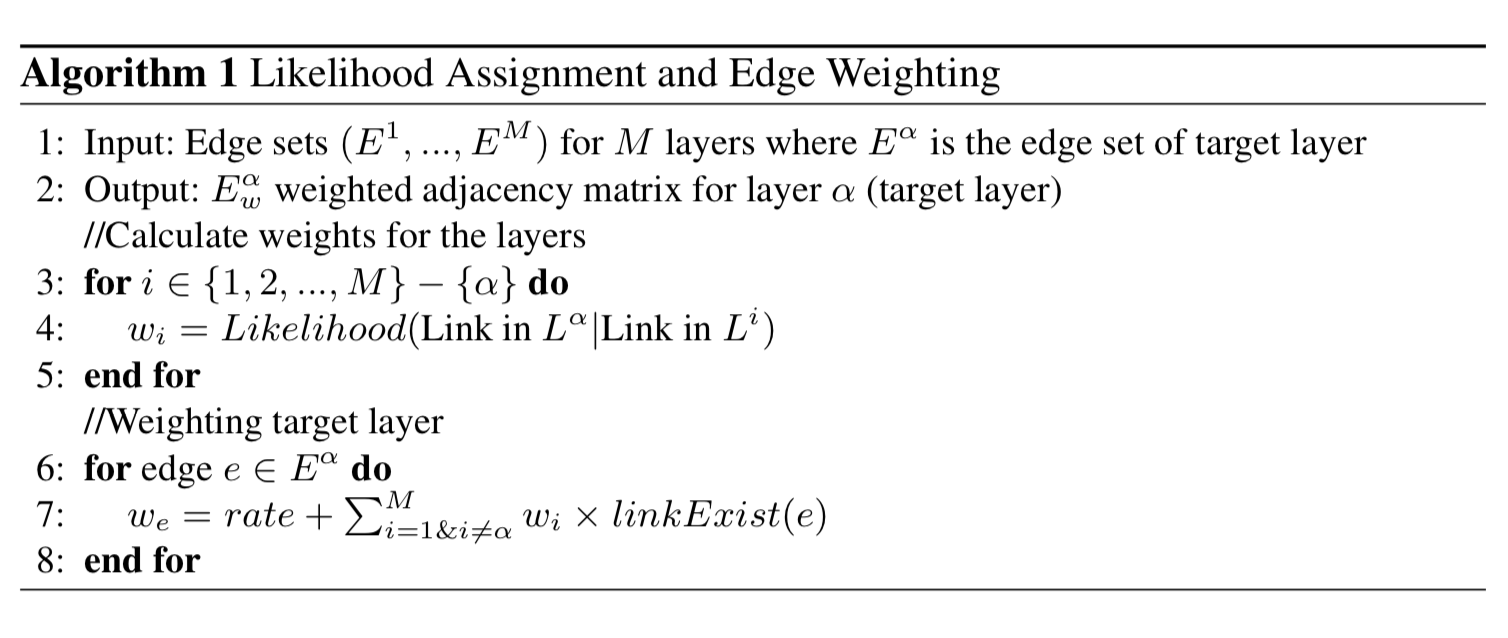
\includegraphics[width=\linewidth]{pics/algo1.png}  
\caption{Reweighting the edges of a target layer}
\label{fig:algo1} 
}
\end{figure}

The algorithm implements reweighting of edges in the target layer for which we
need  to predict links. The reweighting is done by assigning a weighted score
between the  target layer and other layers, in this case cardinality of the
intersection between two  layers. The term \texttt{rate} is the average of a
source node's out-degree over previous timestamps. Function \texttt{linkExist}
returns  $1$ if a link exists in that layer, in any of the past snapshots.
After reweighting, they use similarity metrics described in
section~\ref{sec:slp} on the reweighted graph and finally use Borda's rank
aggregation on different similarity metrics to predict the links for the
current layer. In this paper we introduce a modified version of
algorithm~\ref{fig:algo1} and compare  this with the original one.




% A paragraph or two about multi layer link prediction and methods used previously.














